\documentclass[10pt,a4paper]{article}
\usepackage[latin1]{inputenc}
\usepackage{amsmath}
\usepackage{amsfonts}
\usepackage{amssymb}
\usepackage{hyperref}
\usepackage{graphicx}
\usepackage{cite}
\usepackage[table]{xcolor}
%\usepackage[style=nature, backend=biber]{biblatex}
%\addbibresource{./bibfile.bib}
\DeclareMathOperator*{\argmax}{argmax} % no space, limits underneath in displays

\begin{document}
	\title{Natural Language Processing for tasks with specialized domain language  --  Project Report}
	\author{data.camp097@audi.de}
	\maketitle
	\tableofcontents
	\section{Definition}
	
	
	\subsection{Overview}
	Natural Language Processing as a sub-discipline of machine learning has had major success in recent years on a broad range of problems. 
	Many natural language related task in the industry are however not yet automated. As an example, in the automotive industry these tasks comprise automated scanners for the monitoring of (social) media with respect to potential quality or safety problems (a legal requirement for manufacturers), automated analysis of warranty and repair documents, systems for customer support, monitoring and analysis of patent applications to identify trends and many more. One of the main hurdles for automation of these spezialized tasks has been performance: 
	When confronted with highly specialized sub-domain languages like automotive engineering, commercial off the shelf (COTS) products decline in performance, often up to a point of being useless \cite{OilandGas}. 
    

	\subsection{Problem Statement}
	
	One key element of many NLP pipelines are word embeddings, dense vecor representations of the vocabulary. Examples of these methods are word2vec \cite{word2vec}, GloVe \cite{pennington2014glove} or FastText \cite{bojanowski2017enriching}. These word embeddings are able to represent (surprisingly) much semantic and syntactic meaning, which makes downstream NLP tasks in general much easier. However, to learn this, the embeddings have to be trained extensively, state of the art are data corpora with tens of billions of tokens. When it comes to specialized sub-domain language, data is in general not easily available, often proprietary, confidential or copyright protected and never as abundant as general text. 
	The basic hypothesis for this capstone project is the assumption that the dominant problem of NLP algorithms operating on specialized domain languages is the fact that during training the algorithm hasn't seen any or enough domain specific text. For this reason I trained two different vector representations, the classic word2vec and the more recent FastText on a self-aquired domain specific data corpus and compared it with different metrics to a generic model, the Facebook German Fasttext Model.
		
	\subsection{Metrics}
	\label{eval}
	The evaluation of word embeddings is no easy task. To the best of my knowledge, there does not exist a single commonly used or agreed upon method on how to evaluate these models\cite{1901.09785, Schnabel15, 1801.09536}. Instead a range of methods is used. These methods fall in two categories, extrinsic and intrinsic. Intrinsic evaluation takes into consideration only the embedding itself whereas extrinsic methods measure the embedding performance indirectly by a downstream NLP task with its own metric. For this project, I implemented the following metrics to compare the different embedings:
	
	\begin{itemize}
		\item \textbf{$M_1$: Extrinsic measure.} A real world multiclass classification task of software change requests (CRQ) for embedded control software. The classification separates the CRQs by topic to forward it directly to the right experts and change control boards.\footnote{The CRQs themselfes are confidential and cannot be published or submitted.}  
		
		For the classification task, I built an LSTM with the word embedding as a first (untrainable layer). The architecture itself is pretty basic using an attention layer. \footnote{ Adopted from \url{https://github.com/philipperemy/keras-attention-mechanism}}
		The motivation for the attention layer is the fact, that the engineers are encouraged to use a certain structure to describe the CRQ. Therefore it might be possible, to focus the attention to certain areas of the CRQ for classification. 
		
		The model itself can be found in the notebook "LSTM.ipynb".
		
		\item \textbf{$M_2$: Clustering by subsystem.} A vehicle is built from subsystems like engine, transmission, exhaust system, etc.. For 5 subsystems we will pick representative 10 representative words that will represent this subsystem. 
		
		The basic idea of this metric is then to leverage clustering or classification in the vector space of the embedding itself. As the metric for word embeddings is the consine distance, 
		\begin{equation}
		d(\bold{a}, \bold{b})=\cos(\theta)=\frac{\bold{a} \cdot \bold{b}}{|\bold{a}|\cdot|\bold{b}|}
		\end{equation}
		the clustering or classifcation algorithms will have to use this as a measure of distance.
		
		To generate a metric out of this idea, I chose KNN classification with cosine distance and use the train(!) error as the metric. This is motivated by the intuition, that KNN classification only works if the subsystems are tightly grouped and have distance to other clusters. 

		
		\item \textbf{$M_3$: Word analogy.} Another intrinsic metric for word embddings is to assess semantic meaning. We look for relations of the form
		$$ a:b::c:d $$
		In particular, we will assess the semantic representation of technical concepts. Two examples are 
		$$\text{engine : engine control unit :: transmission : transmission control unit}$$
		$$\text{camshaft : camshaft bearing :: crankshaft : crankshaft bearing}$$
		
		We can extract the word d from words a,b and c from the embedding simply with
		\begin{equation}
		d=\argmax_{i} \frac{(x_b -x_a + x_c)^T\cdot x_i}{|x_b-x_a+x_c|}
		\end{equation}
		
		For this to become a metric, I simply count the number of word analogies the embeddings get right in their Top-n list. 
		
		\item \textbf{$M_4$: Word similarity}. A well known metric is the correlation with human similarity scores (like wordsim353...) pairs of words from technical jargon and ask colleagues to rate their similarity. This measure of similarity will then be compared to the cosine distance the embeddings produce for these word pairs. This metric can also be adopted to include relatedness instead of similarity.
		
		\item \textbf{$M_5$: Visualizytions} As a qualitative measure I visualized the embeddings using t-SNE \cite{vanDerMaaten2008} to get a comparative qualitative measure.
		
	\end{itemize}
	
	\section{Analysis}
	\subsection{The Dataset}
	
	For a domain specific data corpus I scraped the text from the following sources:
	\begin{itemize}
		\item technical / specialist books: 60 titles, 28507 pages, 5950125 words in total 
		\item internal technical documentation: 17763 change requests for embedded control software with a total of 960921 words\footnote{proprietary, cannot be submitted} 
		\item patents: 500 patents from the domain vehicle powertrain, containing a total of 9871 pages with a total of 3929993 words.
	\end{itemize}
	
	This data corpus would in principle be easy to scale up by at least two orders of magnitede. As a company, we have access to electronic versions of books from almost all major publishers in the field. Furthermore we have electronic access to the major journals in the field. The patent database is public and with a paid account we can access an unlimited number of documents. The internally available data is of course limited, however only a fraction of the available data was used in this project.      
	 
    \subsection{Algorithms and Techniques}
    \paragraph{Embedding Algorithms}
    The main idea of word embeddings is the representation of the vocabulary by a dense vector representation in a relatively low-dimensional vector space as opposed to the sparse alternatives Bag-of-Words or one-hot encoding. The idea behind this is to capture semantic and syntactic meaning that cannot be represented by the sparse representations.
    
    \paragraph{word2vec} word2vec learns the word embeddings with one of two methods (see figure \ref{w2v}\footnote{https://towardsdatascience.com/an-implementation-guide-to-word2vec-using-numpy-and-google-sheets-13445eebd281}):
    \begin{itemize}
    	\item CBOW Model: This method takes the context of each word as the input and tries to predict the word corresponding to the context. 
    	\item Skip-Gram: This method takes a target word and tries to predict the words in the context.
    \end{itemize}
    Both methods use neural nets to learn, the basic structure for CBOW is depicted in figure \ref{w2v_arch}\footnote{\url{https://towardsdatascience.com/introduction-to-word-embedding-and-word2vec-652d0c2060fa}}
    
\begin{figure}
    \begin{center}
    	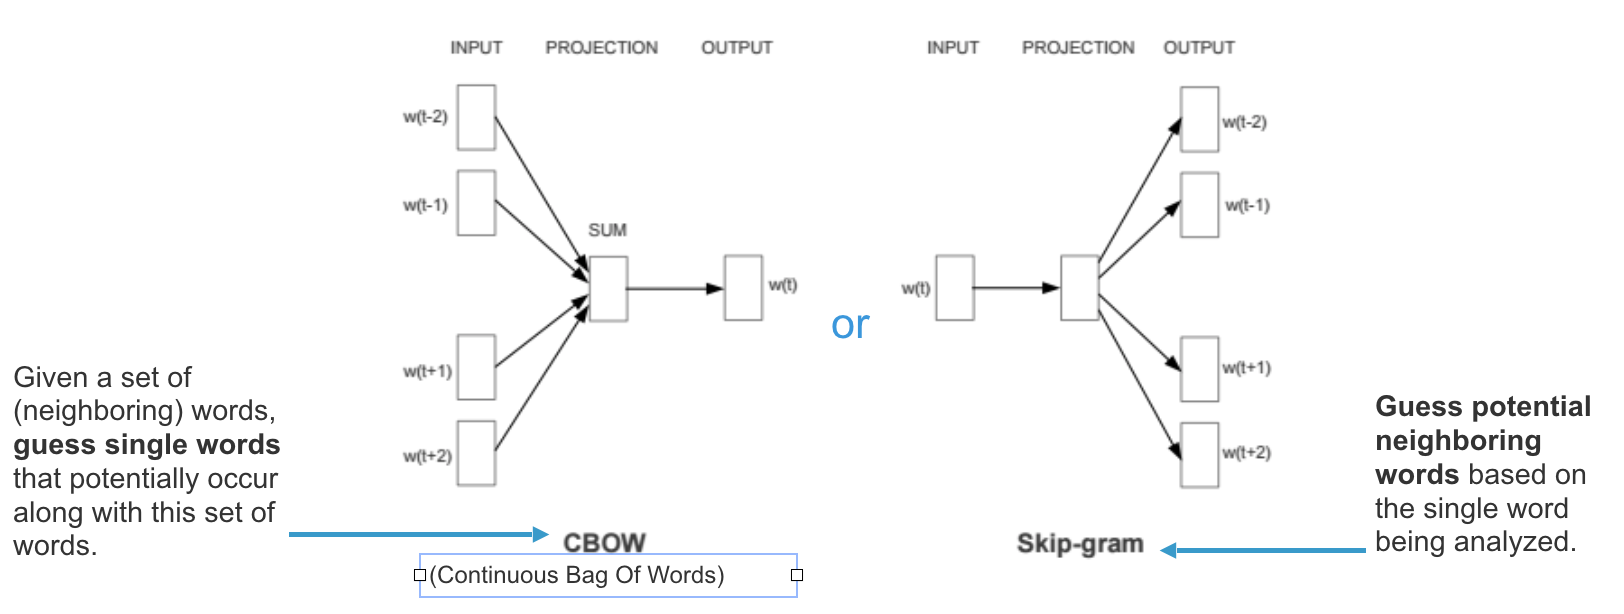
\includegraphics[scale=0.25]{./Pictures/w2v_pic.png}
    	
    	\caption{The basic idea of word2vec}
    	\label{w2v}
    \end{center}
\end{figure}

\begin{figure}
	\begin{center}
		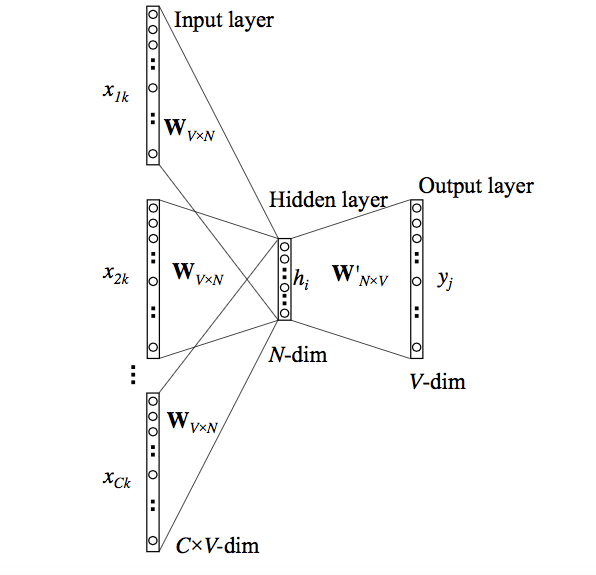
\includegraphics[scale=0.4]{./Pictures/w2v_arch.png}
		
		\caption{The basic network architecture from word2vec CBOW}
		\label{w2v_arch}
	\end{center}
\end{figure}

    \paragraph{FastText} FastText extends word2vec. It is built on character n-grams, whereas word2vec takes whole words as the smallest units. This property should give FastText an advantage with rare words and especially with German compound nouns.
    
    \paragraph{Evaluation Techniques}
    The techniques used to evaluate the are described in section \ref{eval}.
    
    
    \subsection{Benchmark Models}
    As a benchmark I chose the pretrained German Facebook FastText embedding. \footnote{\url{https://fasttext.cc/docs/en/crawl-vectors.html}} This model is trained on German Common Crawl and Wikipedia Data (in the range 10-100 billion tokens).
			
	\section{Methodology}
	
	During the implementation I tried to use existing packages as much as possible. For NLP related tasks these were gensim \cite{rehurek_lrec}, NLTK \cite{Loper:2002:NNL:1118108.1118117} and spacy \cite{spacy2}. For machine learning related tasks, these were Keras, TensorFlow and scikit-learn.
	
	
	\subsection{Data Preprocessing}
	For the preprocessing, the following steps were taken:
	\begin{itemize}
		\item Scraping raw text from pdf. This is done with the Python packages "textract" and "PyPDF2". Used on the patents and the books, the CRQs were scraped directly to raw text via SQL from a database.
		\item The structure of the data is a list of lists, the inner lists being the scope over which the windows run while training.
		\item The raw text is serialzied to disk using pickle.
		\item The raw text is stripped of punctuation, numerics, multiple whitespace, words shorter than 3 letters, and German stop words. It is lower-cased and split. A lemmatizer was integrated but not used due to runtime considerations. The list of German stop words was imported from the python package "get\_stop\_words", the preporcessing was mainly done with the package "gensim" preprocessing functions.
		\item The preprocessed text is serialized to disk using pickle,
	\end{itemize}
    The scraping and preprocessing is implemented in the notebook "Data Collection.ipynb". 
    
	\subsection{Embedding Training}
	
	Training the embeddings was done using the package "gensim". 
	
	\begin{verbatim}
		model_w2v = Word2Vec(training_data, size=300, window=5, min_count=5)
		model_ft = FastText(training_data, size=300, window=5, min_count=5)
	\end{verbatim}
	
	The main parameters of the embedding are the size of the embedding vector space, which I set to 300, and the window size, which defines the number of words in the context, to 5. Both pretty much default values.
	The training of the embeddings is implemented in the notebook "Embeddings.ipynb"
	
	
	\subsection{Evaluating the Embeddings}
	
	The metrics are described in section \ref{eval} Implementation relied as much as possible on existing packages like keras, scikit-learn and gensim. The results are discussed in section \ref{results}.
	
	
	The evaluation metrics are implemented in the notebooks "LSTM.ipynb" and "Metrics.ipynb"
	
	
	
	\subsection{Optimization}
	
	\paragraph{Optimizing the embeddings}
	To optimize the embeddings, a few options are available.
	\begin{itemize}
		\item Embedding parameters. I used "default" emedding parameters, vector space dimensions of 300 and context window size of 5. It might be worthwhile to experiment with these parameters.
		\item More training data: As the training data is unlabelled, it is feasible to massively increase the amount of domain specific training data. I would assume that at least a factor of 100 would be possible.
		\item Using different embedding algorithms. So far, I used only 2 widely used algorithms, word2vec and FastText, but there are many more established algorithms with will documented strengths and weaknesses. It might be worthwhile to see if improvements could be made by choosing more wisely.
		\item Retraining a pretrained network. For some embedding algorithms it is possible to retrain them on additional data. It would be interesting to measure the performance of a retrained embedding and compare the results to the exclusively trained embeddings used in this project. In theory it might be possible to somehow bring the good general performance and the domain specific training together.
	\end{itemize}
	
	
	\paragraph{Optimizing the classifier}
	\label{opt_class}
	Even though the classifier is mainly used as a metric to evaluate the different embeddings, some very basic optimization was done before using it. The overall goal is to prevent overfitting and increase test accuracy. 
	
	The networt currently still seems to overfit, see figures \ref{acc} and \ref{loss}. This is not surprising considering the very small number of available labelled samples and the relatively large capacity of the network.
	\begin{figure}
		\begin{center}
			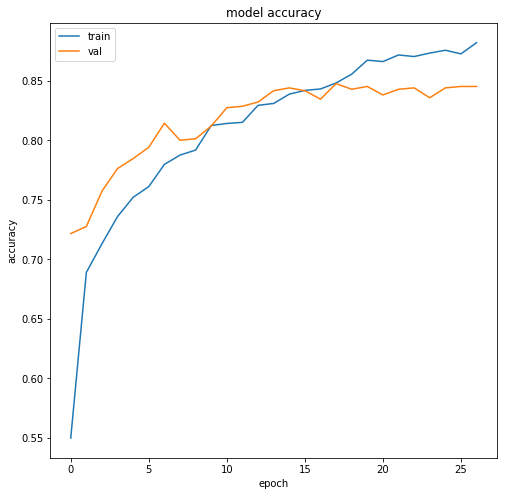
\includegraphics[scale=0.4]{./Pictures/m_acc_ds_ft.png}
			
			\caption{Model accuravy while learning with domain specific FastText Embedding}
			\label{acc}
		\end{center}
	\end{figure}
	
	\begin{figure}
		\begin{center}
			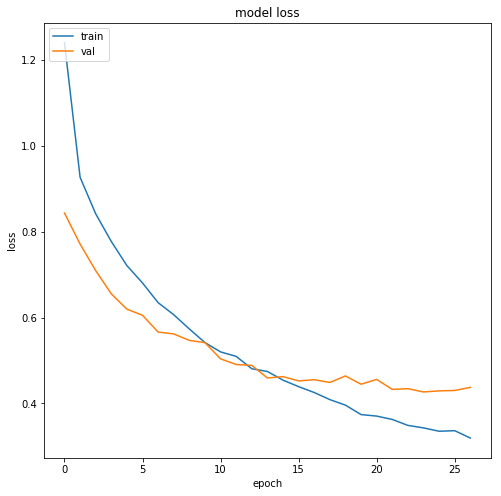
\includegraphics[scale=0.4]{./Pictures/loss_ds_ft.png}
			
			\caption{Loss while learning with domain specific FastText Embedding}
			\label{loss}
		\end{center}
	\end{figure}
	
	
	To prevent overfitting, the following steps were taken:
	\begin{itemize}
		\item Early termination was implemented in the learning. 
		\item Dropout was applied extensively through the network (between layers and recurrently inside the LSTM layer). Dropout rate used is 0.4 everywhere.
		\item Model Capacity was reduced by decreasing the size of the LSTM internal state to 80)
	\end{itemize}
    Other options that were not thoroughly explored in this project include
	\begin{itemize}
		\item Regularization. Not yet included.
		\item Data augmentation. Cropping might be an option, but was not explored.
		\item Acquisistion of more data. Always an option :-)
	\end{itemize}



	\section{Results}
	\label{results}
	\subsection{Visualizations}
	To get a qualitative impression of what the embeddings learned to represent I produced t-SNE plots for the 20 nearest neighbours of two different word pairs: ('Motor', 'Getriebe') (meaning engine and transmission, respectively) and ('Benzin', 'Diesel') (meaning gasoline and diesel, respectively). 
	
	From an automotive engineer's point of view, these groups of words should be clearly separated as they refer to different subsystems or different classes of internal combustion engines.
	
	The following plots show the degree of separation the embeddings assigned to these groups of words. The specifically trained FastText stands out here as it seems to be able to distinguish between these clusters of words, see figure \ref{tsne1} and \ref{tsne2}. 
	
\begin{figure}
	\begin{center}
		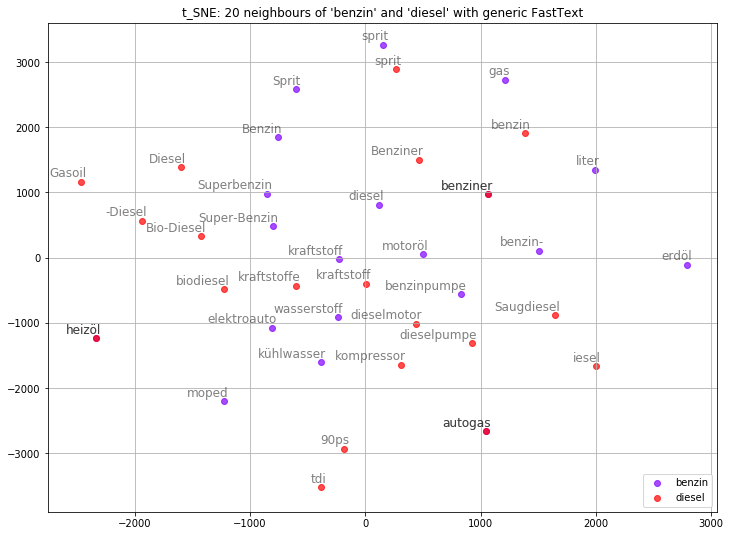
\includegraphics[scale=0.4]{./Pictures/model_ft_benzin_diesel.png}
		
		\caption{t-SNE for generic FastText on word pair ('Benzin', 'Diesel')}
	\end{center}
\end{figure}
	
\begin{figure}
	\begin{center}
	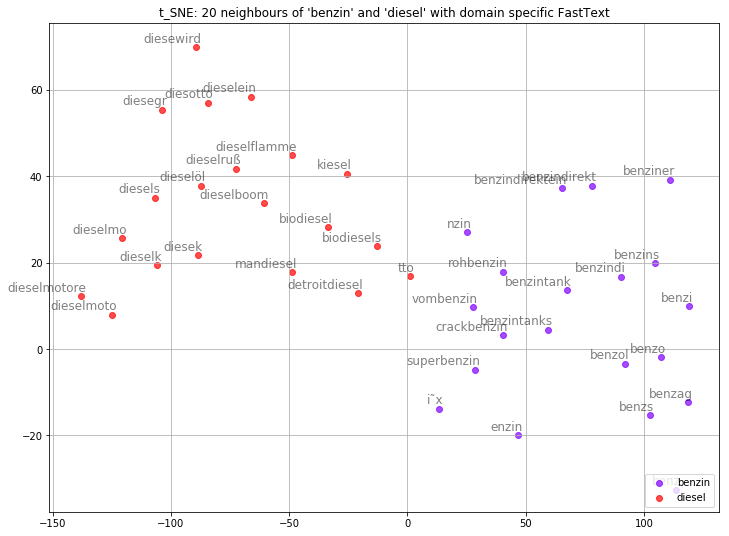
\includegraphics[scale=0.4]{./Pictures/model_ds_ft_benzin_diesel.png}
	
	\caption{t-SNE for domain specific FastText on word pair ('Benzin', 'Diesel')}
	\label{tsne1}
\end{center}
\end{figure}

\begin{figure}
\begin{center}
	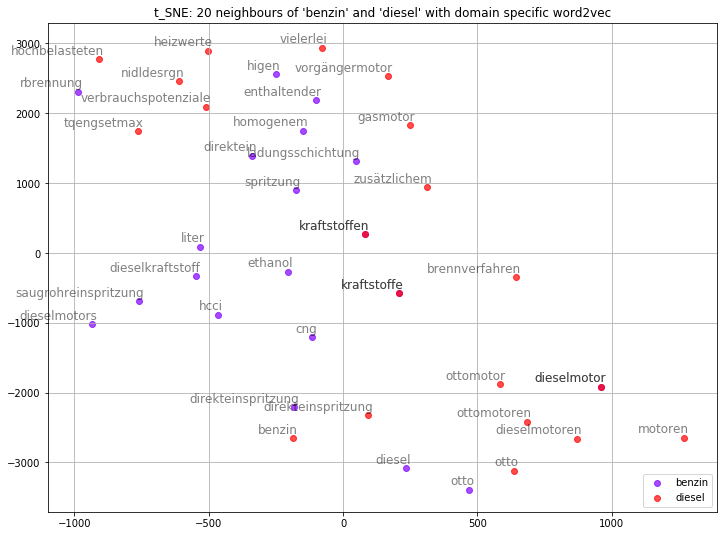
\includegraphics[scale=0.4]{./Pictures/model_ds_w2v_benzin_diesel.png}
	\caption{t-SNE for domain specific wor2vec on word pair ('Benzin', 'Diesel')}
\end{center}	
\end{figure}

\begin{figure}
	\begin{center}
		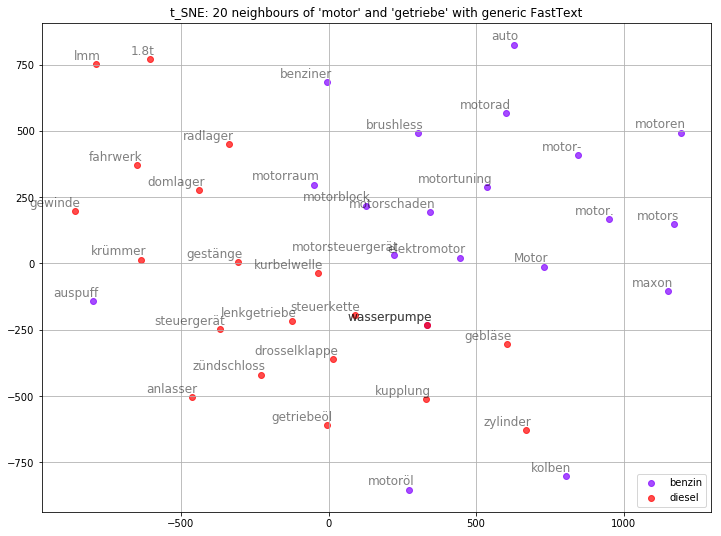
\includegraphics[scale=0.4]{./Pictures/model_ft_motor_getriebe.png}
		
		\caption{t-SNE for generic FastText on word pair ('Motor', 'Getriebe')}
	\end{center}
\end{figure}

\begin{figure}
	\begin{center}
		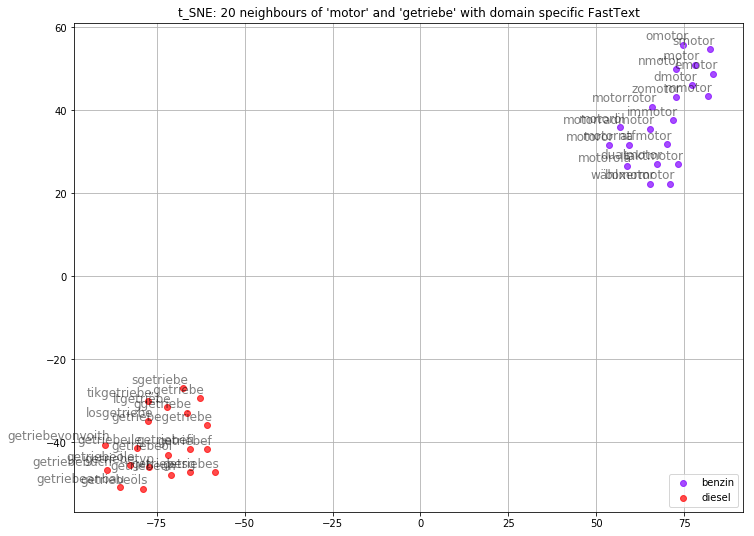
\includegraphics[scale=0.4]{./Pictures/model_ds_ft_motor_getriebe.png}
		
		\caption{t-SNE for domain specific FastText on word pair ('Motor', 'Getriebe')}
		\label{tsne2}
	\end{center}
    
\end{figure}

\begin{figure}
	\begin{center}
		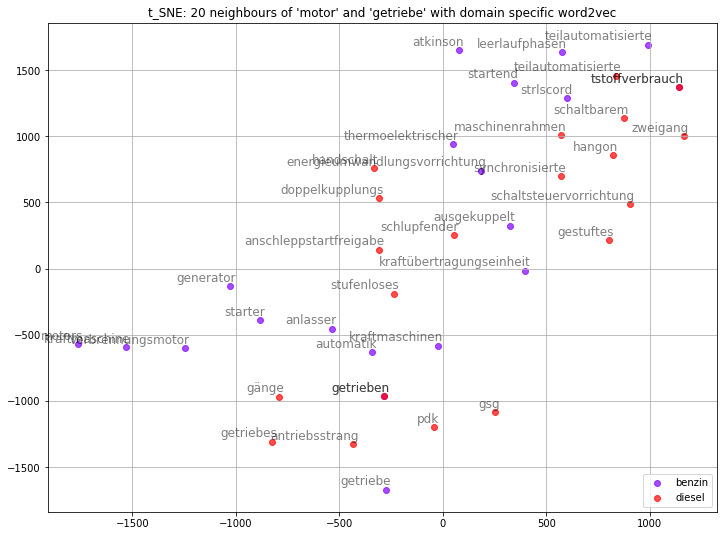
\includegraphics[scale=0.4]{./Pictures/model_ds_w2v_motor_getriebe.png}
		\caption{t-SNE for domain specific wor2vec on word pair ('Motor', 'Getriebe')}
	\end{center}	
\end{figure}

\subsection{Quantitative Results}
\label{quant}
	The metrics \textbf{$M_1$}--\textbf{$M_4$} produce qunatitavie results that are summarized in the following table 
	
	\begin{center}
		\begin{tabular}{|l| c| c| c|c|}
			
			\hline
			
			 & $\boldsymbol{M_1}$ & $\boldsymbol{M_2}$ & $\boldsymbol{M_3}$ & $\boldsymbol{M_4}$\\ \hline
			
			\textbf{Word Embedding} & Test Acc [\%]& Train Acc [\%] & Top-10 & \textsc{Pearson} Corr \\ \hline
		    Generic German FastText   & 80.0 & 67.4 & 0 & -0.28\\  \hline
			
			domain specific word2vec  & 83,6 & 88.4 & 1-Top1,2 & 0.42\\  \hline
			
			domain specific FastText  & 84.5 & 90.7 & 1-Top5  & 0.41\\ \hline 
		
		\end{tabular}
	\end{center}


Before we discuss the results of the metrics, a caveat is in order: The choice of subsystems and subsystem representatives in M$_2$, the choice of word analogies in M$_3$ and the design and assessment of the word similarity list in  M$_4$ would not hold up to any scientific standards. In particular the sample size of all metrics is to small to deliver robust results. Hence the interpretation and discussion of the results is highly speculative.

\paragraph{$\boldsymbol{M_1}$ Downstream Classification}

The results show that the specifically trained word embeddings perform better in this downstream application. This might seem surprinsing, because the generic model is trained on a data corpus 3-4 orders of magnitude larger than the domain specific data corpus used to train the domain specific models. On the other hand, the task needs domain specific knowledge, so a specifically trained model might have an advantage. 
I would like to point out that I did not put much effort in optimizing the architecture, loss function or learning of the classifier. The overall performance for all embeddings could probably be improved significantly (see also section \ref{opt_class}). However, all that is relevant in this context are the relative performances of the different embeddings.

\paragraph{$\boldsymbol{M_2}$ Subsystem Classification in Embedding Space} The results suggest that the embeddings trained on domain specific data can separate the subsystems of the vehicle quite well, whereas the generic model performs significantly worse in this regard. FastText might have an edge over word2vec due to it's property of using character n-grams as the smallest entity, whereas word2vec has complete words as entity. This might help to correctly classify compund nouns. 

\paragraph{$\boldsymbol{M_3}$ Word Analogy}
6 analogies with automotive specific meaning were randomly picked. A point is given for every correctly found analogy in the top-10. Both specifically trained embeddings get one analogy right, whereas the generic embedding does not reproduce any analogy. The word2vec produces the analogy with Top-1 and Top-2 whereas the fasttext embedding gets it with Top-5 only.

\paragraph{$\boldsymbol{M_4}$ Word Similarity} The similarity measure used is a \textsc{Pearson}-coefficient between the human similarity score and the cosine similarity of the embedding. 
The results would suggest, that only the domain specific embeddings capture the similarities, whereas the generic model does not represent any domain specific semantics. This result is to be expected, but would have to be proven in a more rigorous manner.  




\section{Conclusion}
	
By all metrics employed, the generic Facebook FastText model performed worse than the domain specific models. This is remarkable, because the data corpus used to train the generic embedding	is of the size 10s to 100s of billion words, whereas we trained the domain specific embeddings on a corpus of a little more than 10 million words, three to four orders of magnitude smaller.
	
	\subsection{Improvement/Future Work}
	There is much work to be done. From the 9 embeddings I set out to cover, I have implemented 3 (colored in the following table)

	\begin{center}
		\begin{tabular}{|l|p{3cm}| p{3cm}| p{3cm}|}
			\hline
			\textbf{Word Embedding} & pretrained & trained & retrained \\ 
			\hline
			word2vec  & gensim Standard & \cellcolor{blue!25} gensim Implementation & done w/ gensim implementation \\  
			\hline
			GloVe & gensim Standard &w/ gensim implementation & n.a., needs global cooccurence matrix \\  
			\hline
			FastText & \cellcolor{blue!25 }from Facebook  &\cellcolor{blue!25 } gensim implementation & done w/ undocumented feature in Facebook implementation ???\\
			\hline
      \end{tabular}	
\end{center}

The metrics implemented should in general be valid,  however all 5 would need refinement as already mentionend in the caveat in section \ref{quant} to deliver statistically significant results.

	\subsection {Additional Research Questions}
	Due to time contraints, I didn't touch the additional research questions I raised in the proposal. I still think it would be interesting to follow up on them. 
	\paragraph{Extra Dimesions.} If we retrain a word embedding for a specialized subdomain, do we need to add a few dimensions to the vector space "to make room" for additional semantic concepts? Intuitition would suggest that all existing dimensions are already somehow occupied and new technical concepts would require "new space". So an additional question would be: Do extra dimesions improce the embedding quality? And if so, what semantic meaning can we assign the new dimensions? 
	\paragraph{Compund Nouns.} A distinctive feature of the German language are compound nouns. This holds especially true for technical terms like Nockenwellenlagerungskonzept (cam shaft bearing method). I expect this to be of particular importance to be reflected in the embedding. 
	


\section*{Web Resources}
\label{web_resources}
\begin{itemize}
	\item \url{https://github.com/kudkudak/word-embeddings-benchmarks/blob/master/web/datasets/similarity.py}
	\item \url{https://github.com/Hironsan/awesome-embedding-models}
	\item \url{https://github.com/philipperemy/keras-attention-mechanism}
\end{itemize}



\nocite{*}

\bibliography{Project_Report}
\bibliographystyle{ieeetr}

	
	
\end{document}